% siminos/spatiotemp/chapter/glue.tex
% $Author: predrag $ $Date: 2020-05-22 16:09:57 -0400 (Fri, 22 May 2020) $

%  \section{Combining {\spt} solutions}
%  \label{sect:glue}

%Possible figures
%Idea behind gluing
%schematic for gluing
%step by step gluing in space (multiple figures instead of one)
%step by step gluing in time (multiple figures instead of one)
%various \twots\ resulting from gluing
%general picture of gluing in its extension to fluid dynamics?

In \refsect{sect:tiles} we described a method to use tiles
to find solutions motivated by symbolic dynamics. We can also
apply this technique to any \twots\ even though it's not as
well motivated as combining tiles. Because of this
we can use our library of solutions from \refsect{sect:trawl}
to find even more solutions. Another detail we have not discussed is
how to combine solutions such that the converged combination has
the same symmetry as the initial \twots. For example, we can
combine two shift-reflection invariant \twots\ to find a larger
shift-reflection invariant \twot. We will
now describe the process of gluing \twots\ to find larger \twots.
Instead of allowing any number of \twots\ in the initial combination
(like in tiling) we will only glue a single pair of \twots\ at a
time. Progressively larger \twots\ can be made by iteratively gluing
\twots\ together. This distinction between tiling and gluing is because
in tiling there was symbolic dynamic motivation which allows for
any sized symbolic blocks. It might be better to converge symbolic
subdomains in the tiling procedure but we leave that to future
investigations. Of course we want to mention that similarly to our tiling procedure
there is likely much room for improvement of these numerical methods.

Currently, we always glue solutions with identical symmetries because
the final \twot\ is also assumed to have this symmetry. The rationale
behind this is that (for discrete \spt\ symmetries) the \spt\ Fourier coefficients
exist in subspaces of the full set of \spt\ Fourier coefficients. Therefore,
throughout the entire gluing process we constrain ourselves to
a particular symmetry subspace. This requires the gluing
to be done in a symmetry preserving manner. For discrete symmetries
it is sufficient to work with solution's fundamental domains, \ie, the
\spt\ subdomains that can reproduce the entire \twot\ via
symmetry operations. For example, the fundamental domain
for a reflection invariant solution is half of the spatial domain, because the
other half can be acquired by reflection.
The required decisions to be made before the gluing
process are: which dimension we will use to glue
the \twots\ and which \twots\ to glue.
The choice of the solutions, as
previously stated, are required to have the same symmetry.
Other factors that play a role in this decision
are the \spt\ domain sizes of each \twot.
In practice, the transverse dimension to the gluing direction corresponding
to the boundary between \twots\ should have similar magnitudes.
In other words, imagine we want to
glue two solutions defined on $[\speriod{0},\period{0}]$
and $[[\speriod{1},\period{1}]$ and we choose to glue
in the spatial direction.
Because we have decided to glue in space the discrepancy between
$\period{0}$ and $\period{1}$ cannot be too large lest the initial error will
be large. This error of course results from \twots\ tangent's depending on $\speriod{},\period{}$ so
of course if we only have approximations to $\speriod{},\period{}$ we will
only have an approximation to a \twot\ even though the fields individually correpond
to solutions of \refeq{e-ks}. The difference in
dimensions should be bounded above by some unknown value but in practice
this magnitude of this bound can be quite large. This leniency is once again
ascribed to the efficacy of our numerical methods.
We direct the reader to the results displayed in
    \PC{2019-12-06}{
    References `fig:MNGppo12space\_glue'
    `fig:MNGppo123space\_glue' `fig:MNG\_ppoLargeTspaceglue'
    `fig:MNG\_rpoLargeTtimeglue'
    undefined
    }\PCedit{
??%\reffig{fig:MNGppo12space_glue}
,
??%\reffig{fig:MNGppo123space_glue}
,
?? %\reffig{fig:MNG_ppoLargeTspaceglue},
and
??%\reffig{fig:MNG_rpoLargeTtimeglue}
    }
to get a sense of the possibilities of
this gluing method. We highlight
    \PCedit{
??%\reffig{fig:MNGppo123space_glue}
    }
because
the gluing was successful even though the periods differed by a factor of two.

Now that the general idea is in place we shall proceed to explain
the numerical steps in the \twot\ gluing process.
The search for \twots\ in \refsect{sect:trawl} and the tilings of \refsect{sect:tiles}
has already shown that the initial condition can afford to be inaccurate.
There are two main contributions to the error just like the tiling process:
discontinuities at the gluing boundaries and incorrect tangent magnitudes
from errors in $[\speriod{},\period{}]$.
First we perform the usual spectral padding to interpolate a much finer
{\spt} grid so that any cutting and pasting is more precise.
The interpolation is also performed in such a
manner such that their discretizations respect the aspect ratios of
the initial \twots.
That is to say, if one solution is twice as long
(in either space or time) as the other, then the longer solution will have
twice as many discretized point in that dimension. Mathematically
it's the simple relation $\frac{\period{i}}{\period{j}}=\frac{\period{N_i}}{\period{N_j}}$.
If the solutions have continuous symmetry then we are also free to perform
\spt\ rotations such that the difference between the boundaries is minimized.
Spatial rotations are not afforded by solutions with discrete reflection
and shift-reflection symmetries because of the reflection axis.
For these solutions with discrete symmetry we can, however, work with
fundamental domains and then reproduce the full glued \twot\ by
symmetry operation. For reflection invariant \twots\ this corresponds
to taking half of the spatial extent and for shift-reflection invariant
\twots\ it is half of the temporal extent. This
subdivision into and subsequent selection of reflection equivariant subdomains
allows us to construct the approximate fundamental domain of our new \twot.
Numerically, this new fundamental domain is formed by conjoining
the two initial fundamental domains in physical space by concatenating
the two dimensional arrays containing the field information.
To produce the best initial condition as determined by the
cost functional \refeq{e-costfunctional} we also have to take
the ordering of the fundamental domains in account. The combination
which has the smallest value of the cost functional is taken to be the
representative of this particular gluing.
In case its not clear what is meant by combinations
we will explain with an example. There are eight ways of
combining two fundamental domains
with reflection symmetry. These eight combinations arise
from the spatial ordering as well as which fundamental domains to choose from
the original \twots.
The fundamental domains of each initial \twot\ are equivalent conceptually
but not numerically; it matters which is chosen to be combined.
Once the original \twots\ or fundamental domains therefrom are combined,
we apply a smoothing procedure to create a better initial condition.
The smoothing is handled by truncating the high frequency \spt\ \Fcs.
This is a simple way
of reducing the effect of the Gibbs phenomenon; the effect of the boundary
discontinuities on the \spt\ \Fcs. Other possible methods are
mentioned in \refsect{sect:tiles} and so are not repeated here. The main
takeaway is that the numerical methods seem effective enough to not
warrant a complicated procedure to combine solutions.
Still, this added effort has currently not been worth
pursuing due to the strength of the developed numerical methods, but
it is good to keep an additional procedure handy if our goals
change and require better initial conditions.
The gluing of \twots\ and fundamental domains of \twots\ are shown
schematically in \reffig{fig:MNGspaceglue}, \ref{fig:MNGtimeglue},
\ref{fig:MNGreflxglue}, \ref{fig:MNGshiftreflxglue} and \ref{fig:MNGshiftrefltglue}.


\begin{figure}
\begin{minipage}[height=.1\textheight]{.45\textwidth}
\centering
\small{\texttt{(a)}} \\
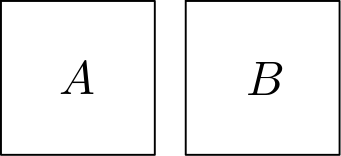
\includegraphics[width=.45\textwidth,height=.07\textheight]{MNG_AB}
\end{minipage}
\begin{minipage}[height=.1\textheight]{.45\textwidth}
\centering
\small{\texttt{(b)}} \\
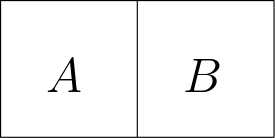
\includegraphics[width=.45\textwidth,height=.07\textheight]{MNG_ABx}
\end{minipage}
\caption{ \label{fig:MNGspaceglue}
Depiction of spatial gluing for \twots\ with spatial translation symmetry.
(a) Initial \twots\ and (b) \twots\ with correct gluing order.
}
\end{figure}


\begin{figure}
\begin{minipage}[height=.1\textheight]{.45\textwidth}
\centering
\small{\texttt{(a)}} \\
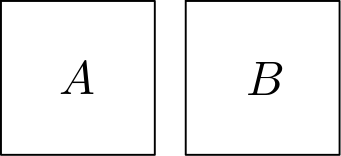
\includegraphics[width=.45\textwidth,height=.07\textheight]{MNG_AB}
\end{minipage}
\begin{minipage}[height=.1\textheight]{.45\textwidth}
\centering
\small{\texttt{(b)}} \\
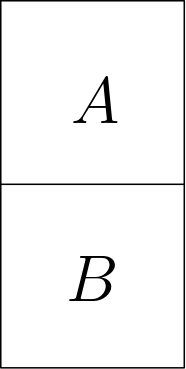
\includegraphics[width=.225\textwidth,height=.15\textheight]{MNG_ABt}
\end{minipage}
\caption{ \label{fig:MNGtimeglue}
Depiction of temporal gluing for \twots\ with either spatial translation symmetry
or reflection symmetry. (a) Initial
\twots\ and (b) \twots\ with correct gluing order.
}
\end{figure}


\begin{figure}
\begin{minipage}[height=.1\textheight]{.45\textwidth}
\centering
\small{\texttt{(a)}} \\
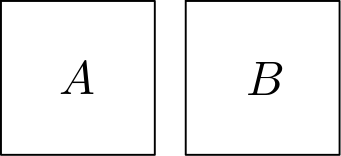
\includegraphics[width=.45\textwidth,height=.07\textheight]{MNG_AB}
\end{minipage}
\begin{minipage}[height=.1\textheight]{.45\textwidth}
\centering
\small{\texttt{(b)}} \\
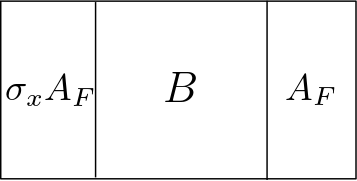
\includegraphics[width=.45\textwidth,height=.07\textheight]{MNG_ABreflx}
\end{minipage}
\caption{ \label{fig:MNGreflxglue}
Depiction of spatial gluing for \twots\ with reflection symmetry. (a) Initial
\twots\ and (b) \twots\ with correct gluing order.
}
\end{figure}


\begin{figure}
\begin{minipage}[height=.1\textheight]{.45\textwidth}
\centering
\small{\texttt{(a)}} \\
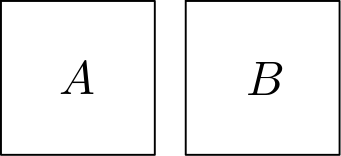
\includegraphics[width=.45\textwidth,height=.07\textheight]{MNG_AB}
\end{minipage}
\begin{minipage}[height=.1\textheight]{.45\textwidth}
\centering
\small{\texttt{(b)}} \\
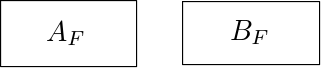
\includegraphics[width=.5\textwidth,height=.035\textheight]{MNG_AFBFshiftrefl}
\end{minipage}
\centering
\begin{minipage}[height=.1\textheight]{.6\textwidth}
\centering
\small{\texttt{(c)}} \\
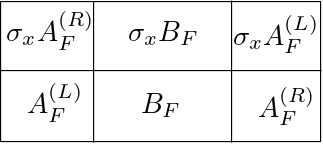
\includegraphics[width=.45\textwidth,height=.09\textheight]{MNG_ABshiftreflx}
\end{minipage}
\caption{ \label{fig:MNGshiftreflxglue}
Depiction of spatial gluing for \twots\ with shift-reflection symmetry. (a) Initial
\twots\ and (b)fundamental symmetry domains (c) post-gluing initial condition for
shift-reflection \twot. Superscripts in this instance stand for ``left'' and
``right'' halves of the corresponding fundamental domain $A_F$
}
\end{figure}

\begin{figure}
\begin{minipage}[height=.1\textheight]{.45\textwidth}
\centering
\small{\texttt{(a)}} \\
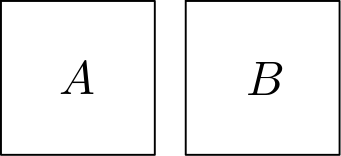
\includegraphics[width=.45\textwidth,height=.07\textheight]{MNG_AB}
\end{minipage}
\begin{minipage}[height=.1\textheight]{.45\textwidth}
\centering
\small{\texttt{(b)}} \\
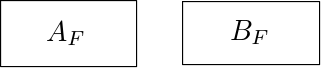
\includegraphics[width=.5\textwidth,height=.035\textheight]{MNG_AFBFshiftrefl}
\end{minipage}
\centering
\begin{minipage}[height=.1\textheight]{.45\textwidth}
\centering
\small{\texttt{(c)}} \\
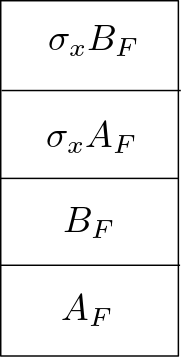
\includegraphics[width=.25\textwidth,height=.20\textheight]{MNG_ABshiftreflt}
\end{minipage}
\caption{ \label{fig:MNGshiftrefltglue}
Depiction of temporal gluing for \twots\ with shift-reflection symmetry. (a) Initial
\twots\ (b) fundamental symmetry domains and (c) post-gluing initial condition for
shift-reflection \twot.
}
\end{figure}

\begin{figure}
\centering
\begin{minipage}[height=.4\textheight]{.66\textwidth}
\centering
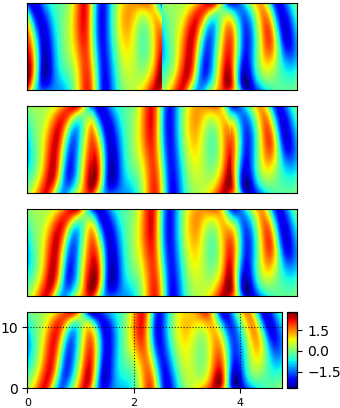
\includegraphics[width=.7\textwidth,height=.6\textheight]{MNGppo12space_glue}
\end{minipage}
\caption{ \label{fig:MNGppo12spaceglue}
Spatial gluing of the two shortest shift-reflection
\twots. The sizes of the fundamental domains of these
\twots\ are
$[\speriod{1},\period{1}]=[3.5\cdots,20.50\cdots]$
and
$[\speriod{2},\period{2}]=[3.5\cdots,28.66\cdots]$
respectively.
The result is a
shift-reflection \twot\ with
$[\speriod{1,2},\period{1,2}]=[6.79\cdots,24.82\cdots]$
fundamental domain.
}
\end{figure}


\begin{figure}
\begin{minipage}[height=.4\textheight]{.99\textwidth}
\centering
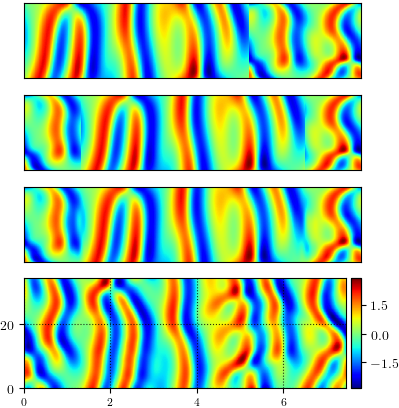
\includegraphics[width=.99\textwidth,height=.66\textheight]{MNGppo123space_glue}
\end{minipage}
\caption{ \label{fig:ppo123spaceglue}
Gluing procedure which spatially combines the third shortest (period) shift-reflection
invariant
$[\speriod{3},\period{3}]=[3.5\cdots,64.70\cdots]$
\twot\
 with the resultant shift-reflection invariant \twot\
from
\PCedit{reffig{fig:ppo12spaceglue}} %2019-12-06
with
$[\speriod{1,2},\period{1,2}]=[6.79\cdots,24.82\cdots]$
fundamental domain.
This results in another shift-reflection
\twot\ with the
$[\speriod{1,2,3},\period{1,2,3}]=[10.53\cdots,68.84\cdots]$
 fundamental domain.
The dramatic change between the last
two panels is presumably an effect of the
discrepancy between the temporal period of
the constituent solutions.
}
\end{figure}
    \PC{2019-12-06}{
    Reference `fig:ppo12spaceglue' undefined in \reffig{fig:ppo123spaceglue}
    }

\begin{figure}
\centering
\begin{minipage}[height=.4\textheight]{.66\textwidth}
\centering
\includegraphics[width=.7\textwidth,height=.6\textheight]{MNG_ppolargeTspaceglue}
\end{minipage}
\caption{ \label{fig:MNGppo12spaceglue1}
Spatial gluing of the two shortest shift-reflection
\twots. The sizes of the fundamental domains of these
\twots\ are
$[\speriod{1},\period{1}]=[3.5\cdots,20.50\cdots]$
and
$[\speriod{2},\period{2}]=[3.5\cdots,28.66\cdots]$
respectively.
The result is a
shift-reflection \twot\ with
$[\speriod{1,2},\period{1,2}]=[6.79\cdots,24.82\cdots]$
fundamental domain.
}
\end{figure}


\begin{figure}
\centering
\begin{minipage}[height=.4\textheight]{.66\textwidth}
\centering
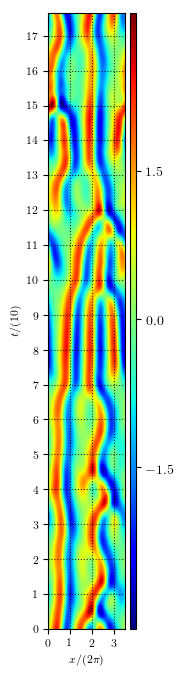
\includegraphics[width=.7\textwidth,height=.6\textheight]{MNG_rpoLargeTtimeglue}
\end{minipage}
\caption{ \label{fig:MNGppo12spaceglue2}
Spatial gluing of the two shortest shift-reflection
\twots. The sizes of the fundamental domains of these
\twots\ are
$[\speriod{1},\period{1}]=[3.5\cdots,20.50\cdots]$
and
$[\speriod{2},\period{2}]=[3.5\cdots,28.66\cdots]$
respectively.
The result is a
shift-reflection \twot\ with
$[\speriod{1,2},\period{1,2}]=[6.79\cdots,24.82\cdots]$
fundamental domain.
}
\end{figure}


    \PC{2019-12-06}{
    Reference `fig:ppo12spaceglue' undefined
    }\PCedit{
refFig{fig:ppo12spaceglue}
    }
and \reffig{fig:ppo123spaceglue}
both demonstrate the spatial gluing
of shift-reflection \twots. In fact, \reffig{fig:ppo123spaceglue}
uses the result of
    \PCedit{
 reffig{fig:ppo12spaceglue}
    }
as an initial
condition. We chose to display these two gluing examples
because they are demonstrative of how gluing can be performed
iteratively to find progressively larger solutions.

\MNG{2019-10-22}{This part is unclear; I'm trying to say that 1-D symbolic
itineraries are much easier to interpret than spatiotemporal blocks...
unfinished and incoherent as of now}

Our tiling and gluing methods constitute ways that larger \twots\
can be found by utilizing smaller \twots. This notion of combinations
has been performed temporally\rf{DV03} as a natural
consequence of symbolic dynamics. In other words, for a dynamical system
with a chaotic attractor it is somewhat straightforward to interpret
symbolic itineraries; they represent visitation of different partitioned
areas of the attractor parameterized with time.
The idea to do this with
respect to spatial dimensions is desirable in the context of minimal
computational cells of plane Couette for instance. Combining solutions
in a \spt\ manner is a whole other beast as symbolic blocks are
hard to interpret in the context of state space.
